\chapter{SPRINT ONE - Manage courses}
\minitoc
\newpage
\section*{Introduction}
\addcontentsline{toc}{section}{Introduction}
In this sprint, we will be developing the authentication system and let the instructors manage their courses.
\section{Sprint backlog}
%%%%%table
\begin{table}[H]
\centering
\caption{Product backlog}
\begin{tabular}{|p{1cm}|p{3cm}|p{6cm}|p{2cm}|}
\hline
\rowcolor{brown!18}\textbf{\large{ID}} & \textbf{\large{As a}} & \textbf{\large{I want to be able to}} & \textbf{\large{Priority}} \\
\hline
1& Instructor  & Access the instructor space & High\\\hline
2& Instructor & Add courses  & High\\\hline
3& Instructor & Delete my courses  & High\\\hline
4& Instructor & Edit my courses  & High\\\hline

\end{tabular}
\end{table}
%%%%%table
\section{Requirement analysis}
\subsection{Use case diagram}

\begin{figure}[!ht]
\centering
     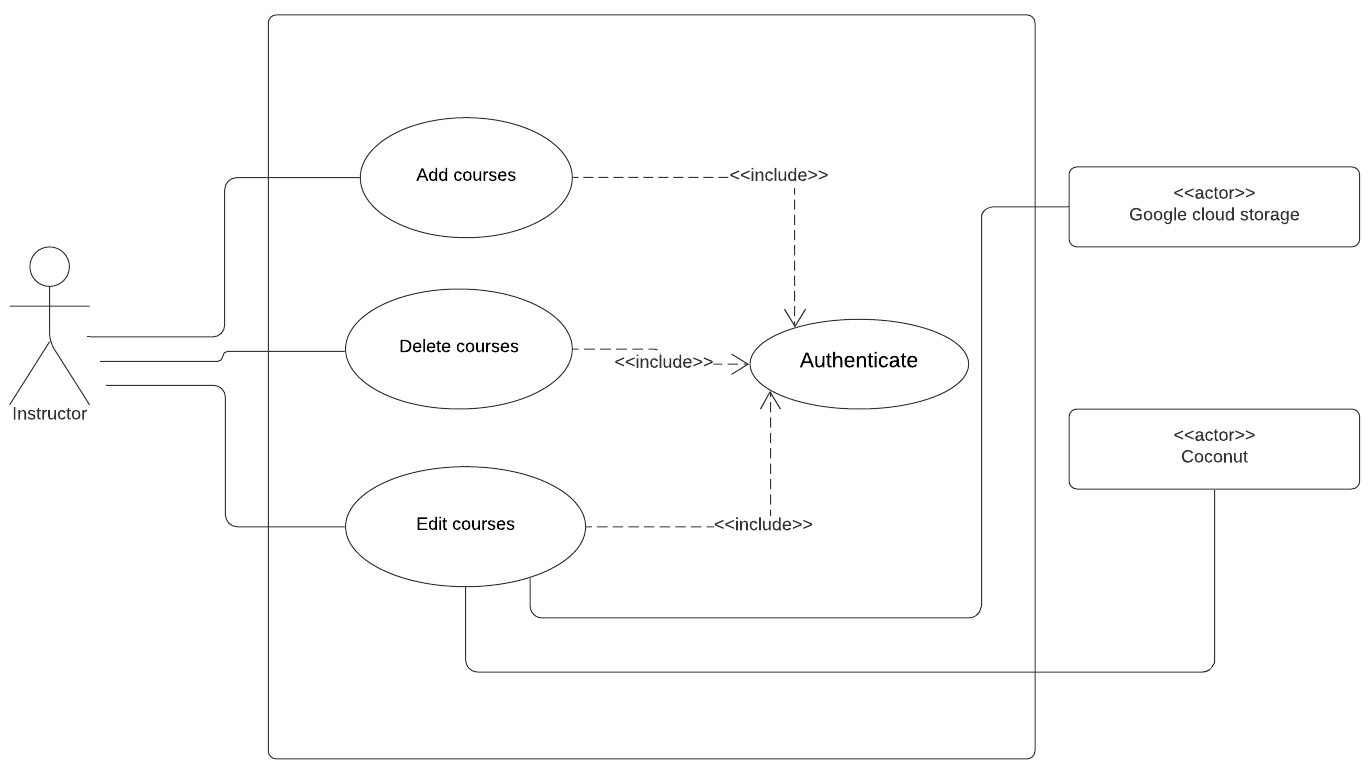
\includegraphics[width=150mm]{sprint1usecase.png}
    \caption{Sprint 1 use case diagram}
    \label{fig:sprint1usecase}
\end{figure}

\subsection{Modeling}

%%%%%table
\begin{table}[H]
\centering
\caption{add courses textual description}
\begin{tabular}{|p{4cm}|p{10cm}|}
\hline
\textbf{\large{Use case name}} & Add courses \\\hline
\textbf{\large{Actors}} & Instructor \\\hline
\textbf{\large{Preconditions}} & User logged in \\\hline
\textbf{\large{Postconditions}} & Course created  \\\hline
\textbf{\large{Normal flow}} & 
\begin{itemize}
  \item The instructor visits the instructor space.
  \item The instructor clicks the courses tab.
  \item The instructor clicks the add a course button.
\end{itemize}
\\\hline

\end{tabular}
\end{table}
%%%%%table

\begin{figure}[!ht]
    \centering
    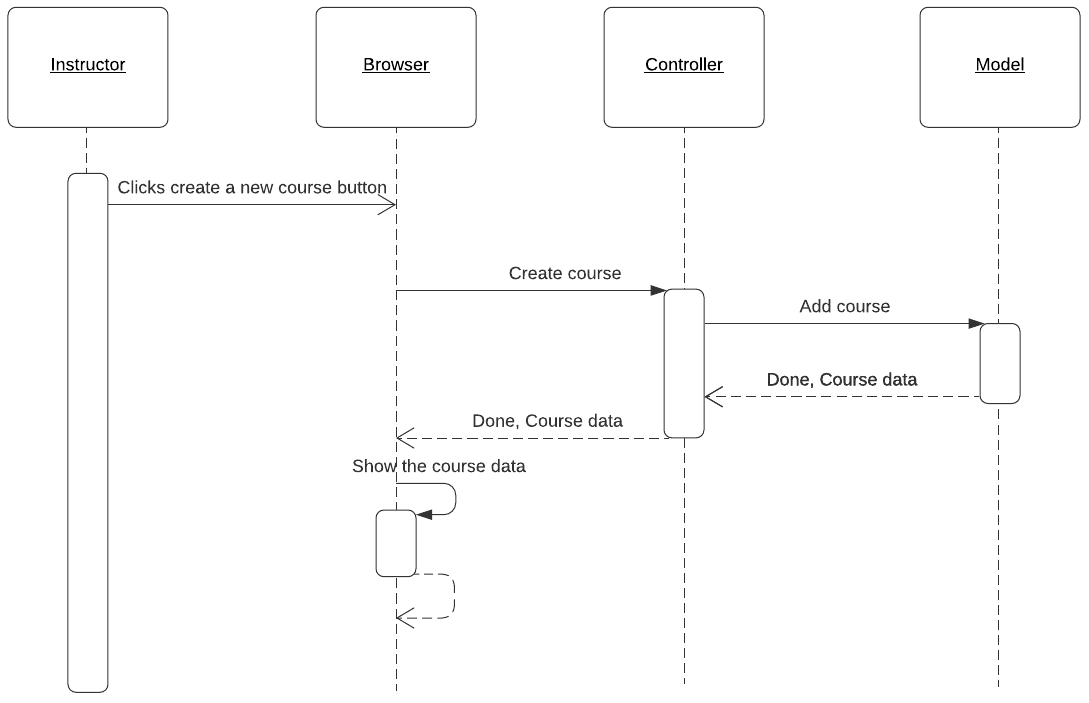
\includegraphics[width=142mm]{seq_create_course.png}
    \caption{Sequence diagram of creating a course}
    \label{fig:seq_create_course}
\end{figure}


%%%%%table
\begin{table}[H]
\centering
\caption{delete courses textual description}
\begin{tabular}{|p{4cm}|p{10cm}|}
\hline
\textbf{\large{Use case name}} & Delete courses \\\hline
\textbf{\large{Actors}} & Instructor \\\hline
\textbf{\large{Preconditions}} & User logged in \\\hline
\textbf{\large{Postconditions}} & Course created  \\\hline
\textbf{\large{Normal flow}} & 
\begin{itemize}
  \item The instructor visits the instructor space.
  \item The instructor clicks the courses tab.
  \item The instructor clicks on the course he wants to delete.
  \item The instructor use the delete button.
\end{itemize}
\\\hline

\end{tabular}
\end{table}
%%%%%table

\begin{figure}[!ht]
    \centering
    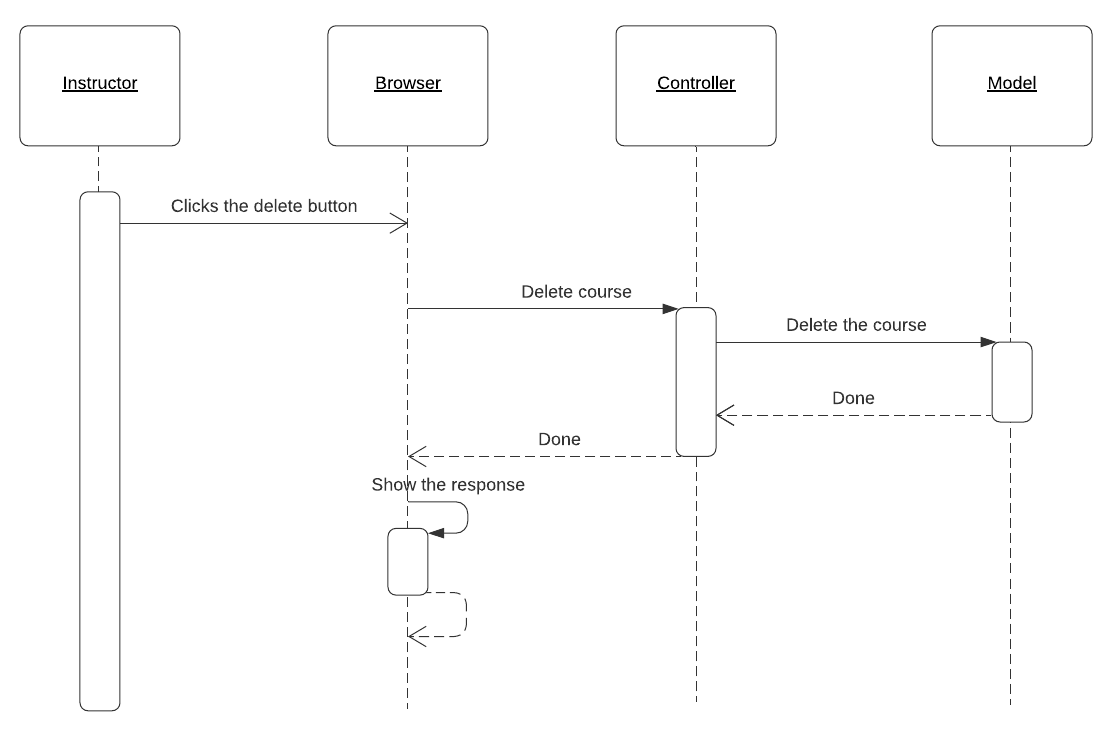
\includegraphics[width=150mm]{seq_delete_course.png}
    \caption{Sequence diagram of deleting a course}
    \label{fig:seq_delete_course}
\end{figure}

\newpage
\vfill

%%%%%table
\begin{table}[H]
\centering
\caption{edit courses textual description}
\begin{tabular}{|p{4cm}|p{10cm}|}
\hline
\textbf{\large{Use case name}} & Delete courses \\\hline
\textbf{\large{Actors}} & Instructor \\\hline
\textbf{\large{Preconditions}} & User logged in \\\hline
\textbf{\large{Postconditions}} & Course edited  \\\hline
\textbf{\large{Normal flow}} & 
\begin{itemize}
  \item The instructor visits the instructor space.
  \item The instructor clicks the courses tab.
  \item The instructor clicks on the course he wants to edit.
  \item The instructor type the meta data of the course.
  \item The instructor save the changes by using the save button.
\end{itemize}
\\\hline

\end{tabular}
\end{table}
%%%%%table

\begin{figure}[!ht]
    \centering
    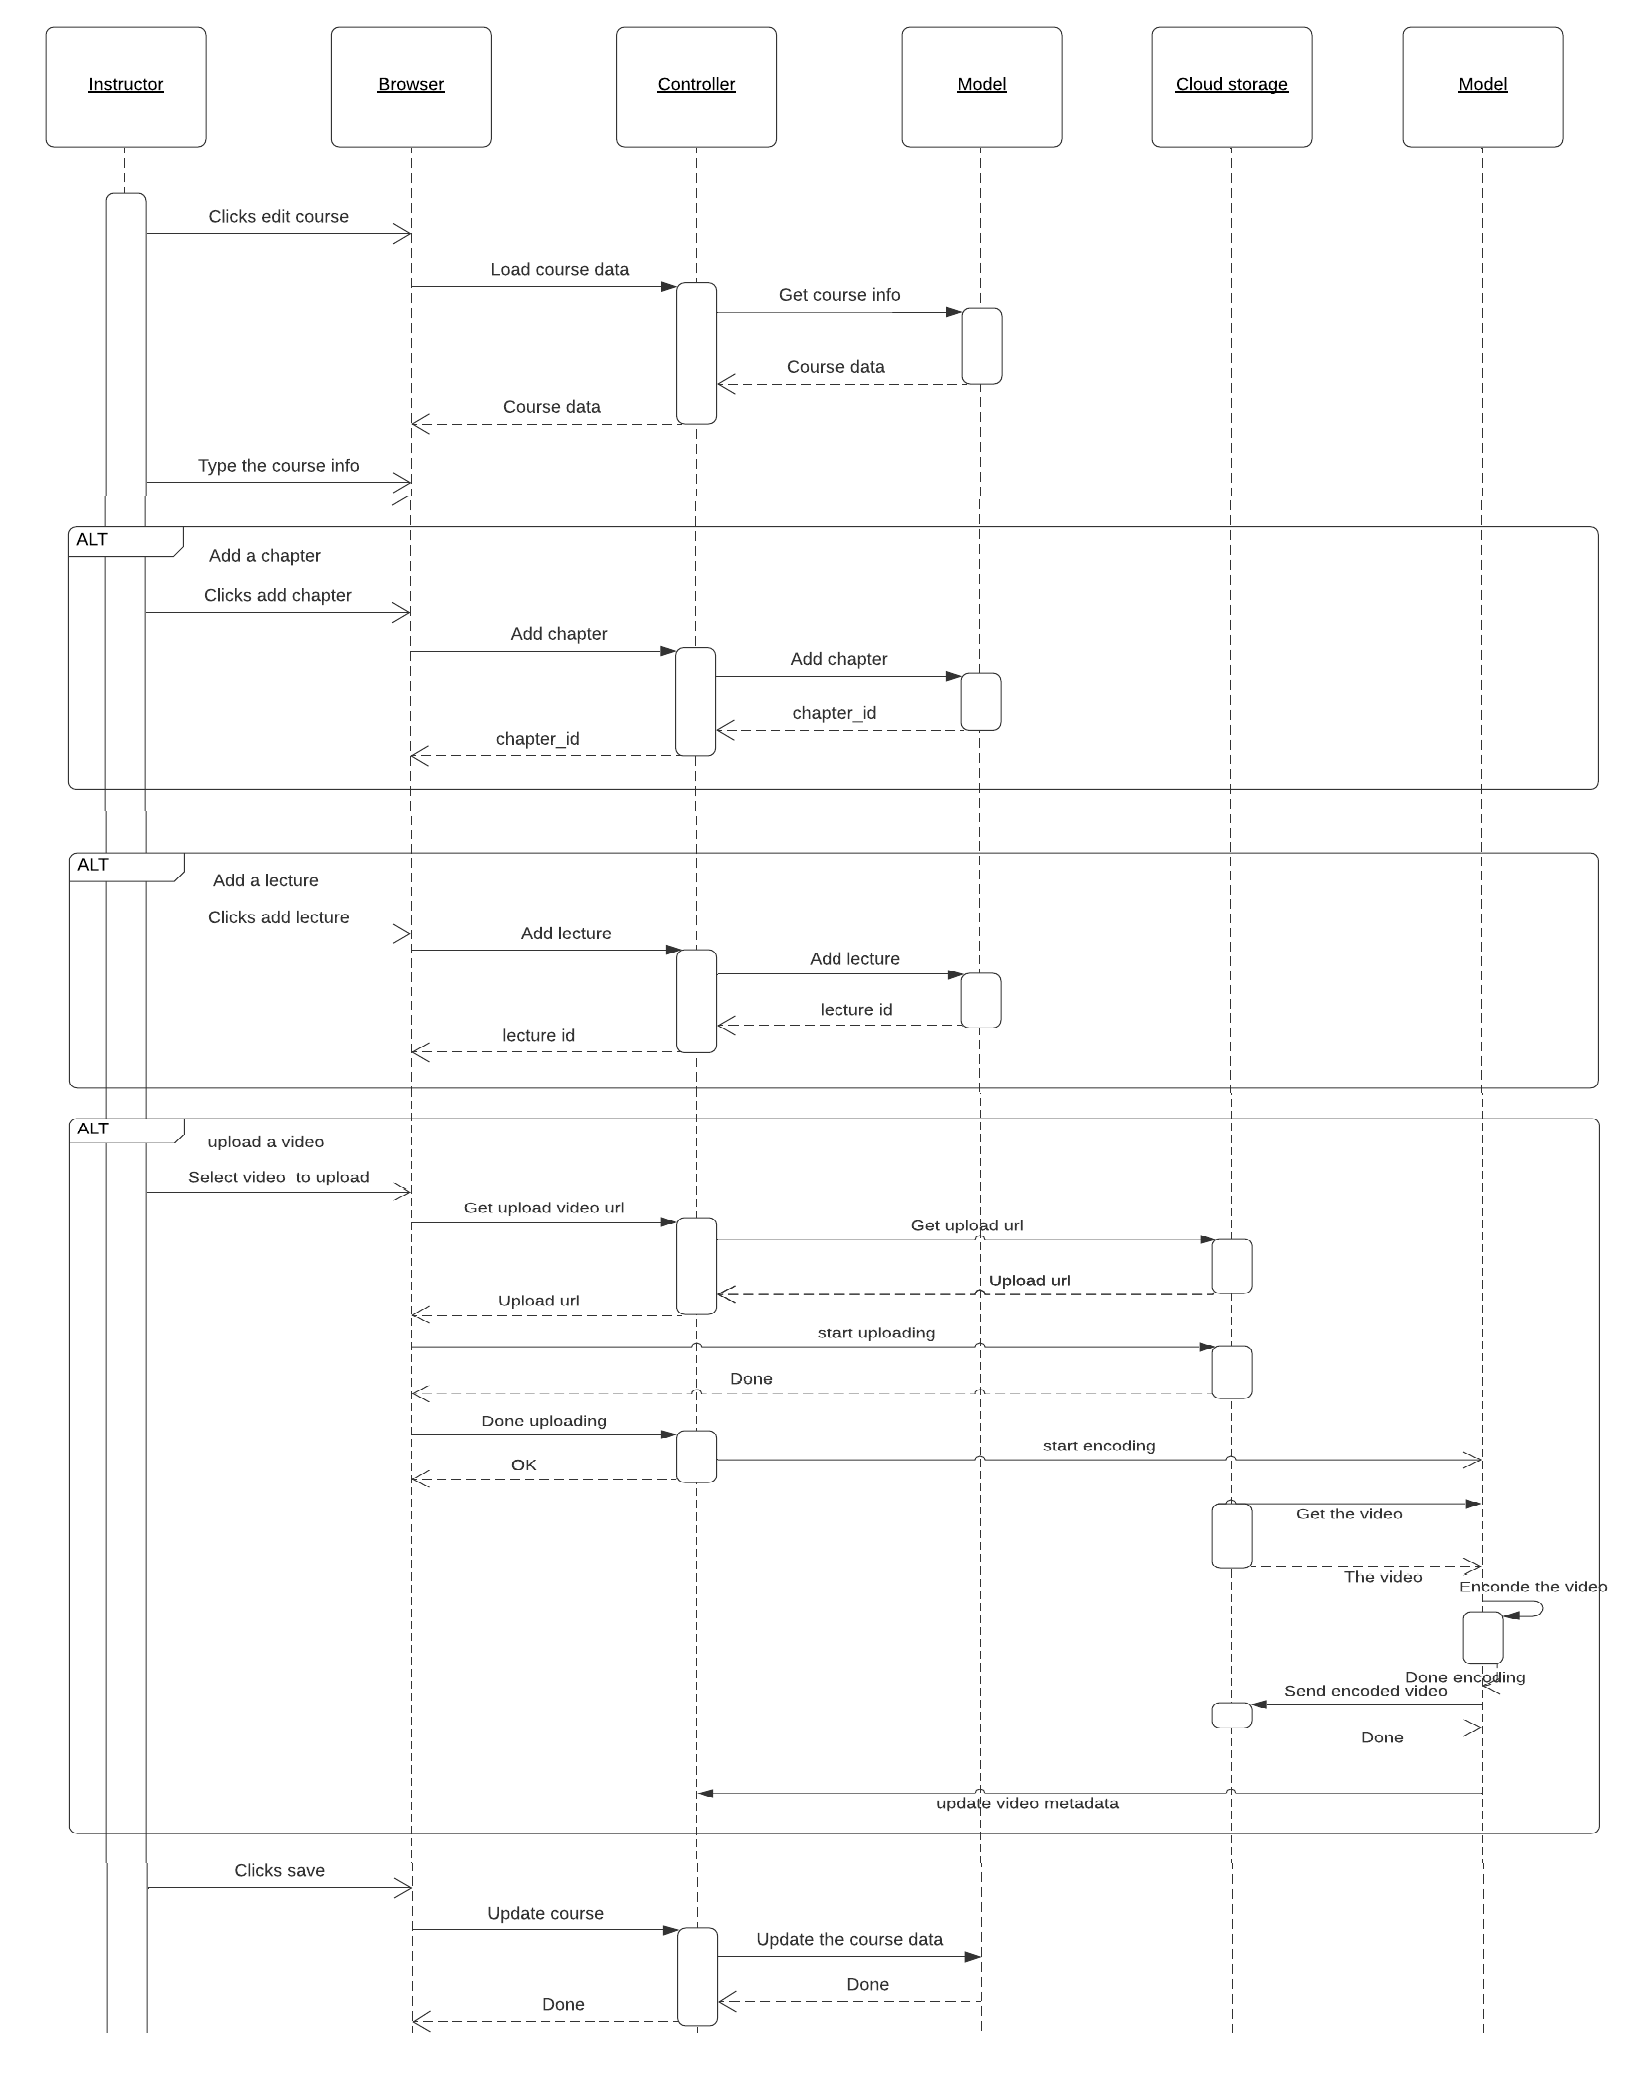
\includegraphics[width=170mm,height=200mm]{seq_edit_course.png}
    \caption{Sequence diagram of editing a course}
    \label{fig:seq_edit_course}
\end{figure}

\vfill
\clearpage

\section{Implementation}

\subsection{Access the instructor space}
As study.tn website already has its own authentication system, the instructor only needs to log in to study.tn then visit the instructor space. Since study.tn and the instructor dashboard are both separate apps, we need to let our app know who's the logged in user in study.tn. Once the instructor tries to visit the dashboard from study.tn we send the authentication token to our dashboard in the url, we get that token, save it in the local storage and then we know who's the user accessing the dashboard with that token.

\subsection{Add a course}
When clicking on the add course button, we make a request to the server to add a new course to the database and as a response we get the created record data (course id, course name...) which is then added to the redux store state to update and re-render the courses.

\subsection{Delete a course}
When clicking on the delete course button, we send a request with the course id to the server to remove the course from the database and show the result of the response to the user accordingly. If no one is enrolled in that course we should recieve a success and remove the course from the redux store to re-render the courses list. 

\begin{figure}[!ht]
    \centering
    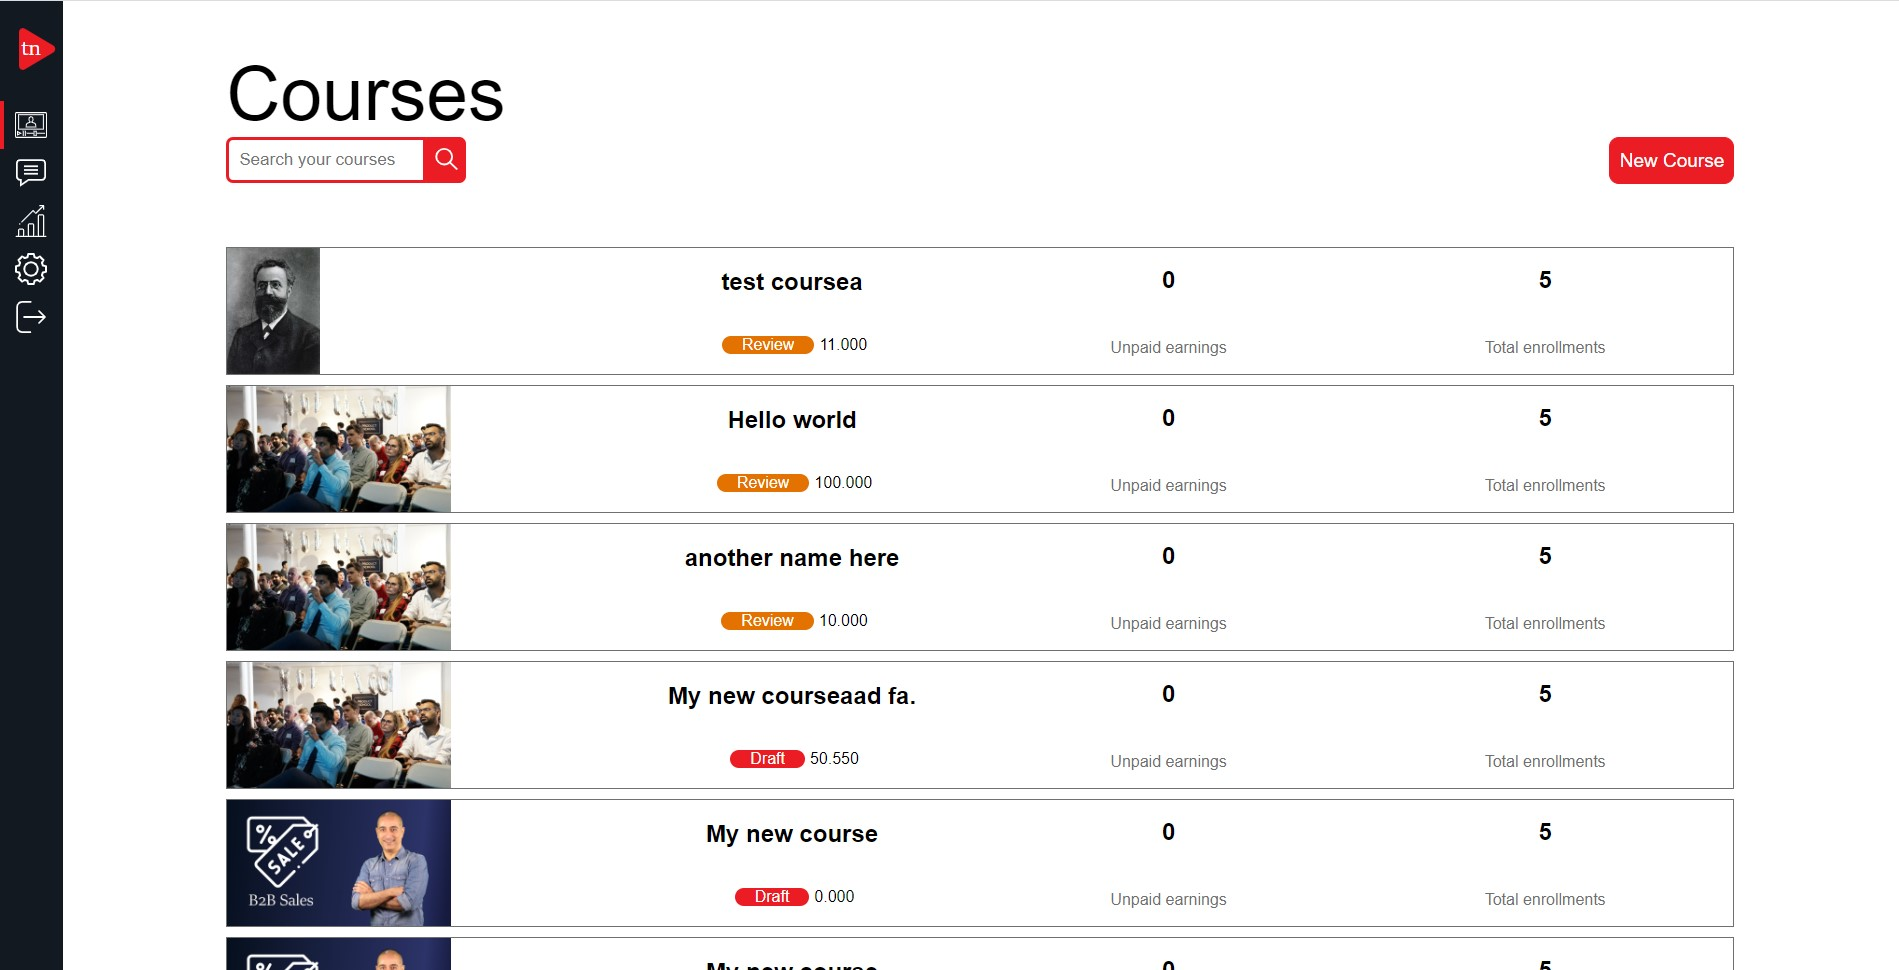
\includegraphics[width=150mm]{courses_tab2.jpg}
    \caption{Courses tab interface}
    \label{fig:courses_tab2}
\end{figure}

\subsection{Edit course}
Clicking on the course in the courses list will bring up a page where the instructor can edit the course and he must fill in the meta data of the course. The page consists of multiple forms each having it's own redux reducer and each form will load it's data individually.

\subsubsection{Target student form}
The instructor writes what are the requirements and prerequisites that students need to have to understand the course in the input field and click the plus button to add it, which will fire a post request to the server sending the text in the input field. When the request is running we show a loader to the user to let him know that something is happening in the background and he needs to wait. After a successful request we update the form state to add the requirement and re-render the form.

\hfill \break
\hfill \break
The instructor can change the order of the requirements list using drag and drop. We implemented it with the help of react-sort-list library which sort the list in the front end, once it's done we make a post request to the server with the requirements new order in the body.
\hfill \break
\hfill \break
We can also delete a requirement by clicking the bin icon and let the server know that we want to delete the element.
\hfill \break
\hfill \break
The process is the same for what will the student learn list.

\vfill
\clearpage

\begin{figure}[!ht]
    \centering
    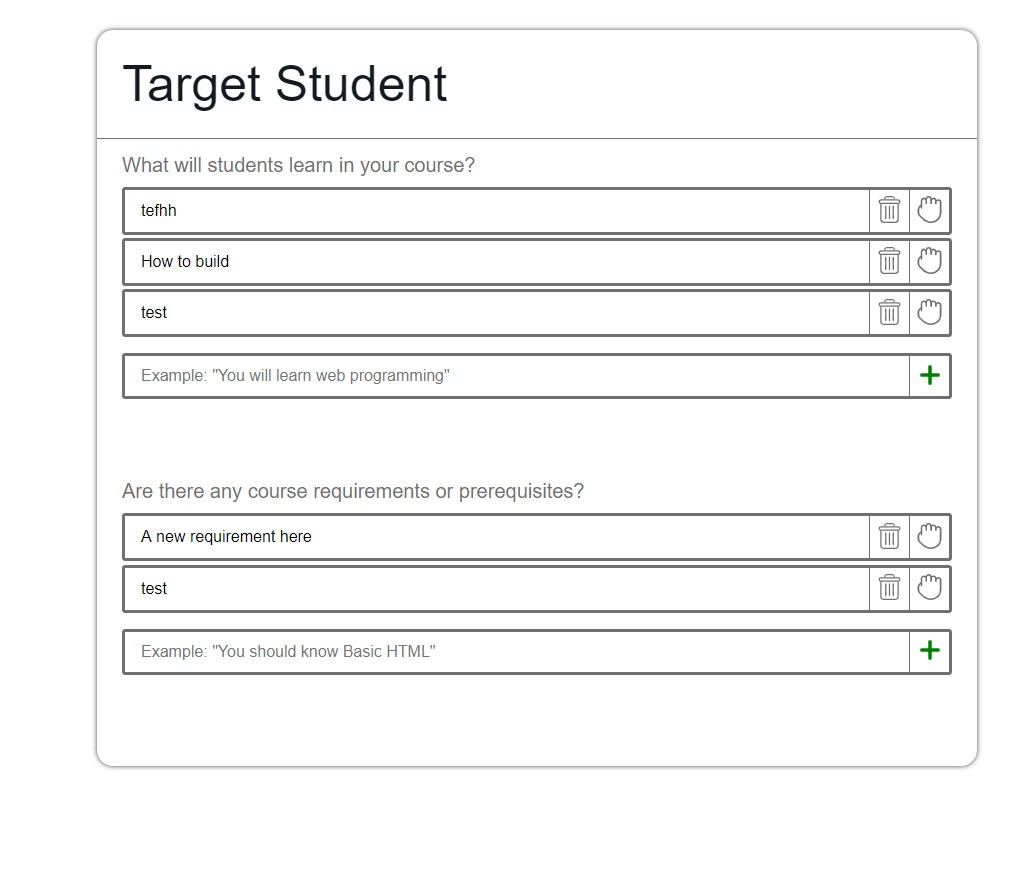
\includegraphics[width=150mm]{target_student_form.jpg}
    \caption{Target student form interface}
    \label{fig:target_student_form}
\end{figure}


\subsubsection{Curriculum form}
A course is composed of chapters, each chapter could have one or more lectures. A lecture is simply a video, but it could have a file as well.
\hfill \break
\hfill \break
We can add a new chapter by clicking add a new chapter button, the browser will make a request to the server and in return we get the created chapter data which we can use to update the redux state and show the new chapter to the user. We can delete a chapter by clicking the bin icon or edit it by clicking the bin icon, let the server know then update the interface. We can also sort the chapter in the same way we did in the target form with the help of react-sort-list library.
\hfill \break
\hfill \break
The same actions performed on chapters can be performed on lectures and they share the same implementation. However, We can upload a video to a lecture by selecting a video, the browser will then make a request to the server to get an upload url and the video id associated to the video that we are about to upload then the upload will start. As the upload process can take time, we show the user a progress bar with a percentage on it. Once it's done we make another request to let the server know that the video has been uploaded successfully and associate the video id with the lecture. Since the video is transcoding and we don't know when this process will end, we refresh the lecture with a random timer between 20 second and 40 seconds to check if the video is ready and show it to the user. The reason behind picking a random timer is to minimize the load on the server so it's less likely that many users will make a request at the same time. The process of uploading a file is as the same as the video except the transcoding phase.

\begin{figure}[!ht]
    \centering
    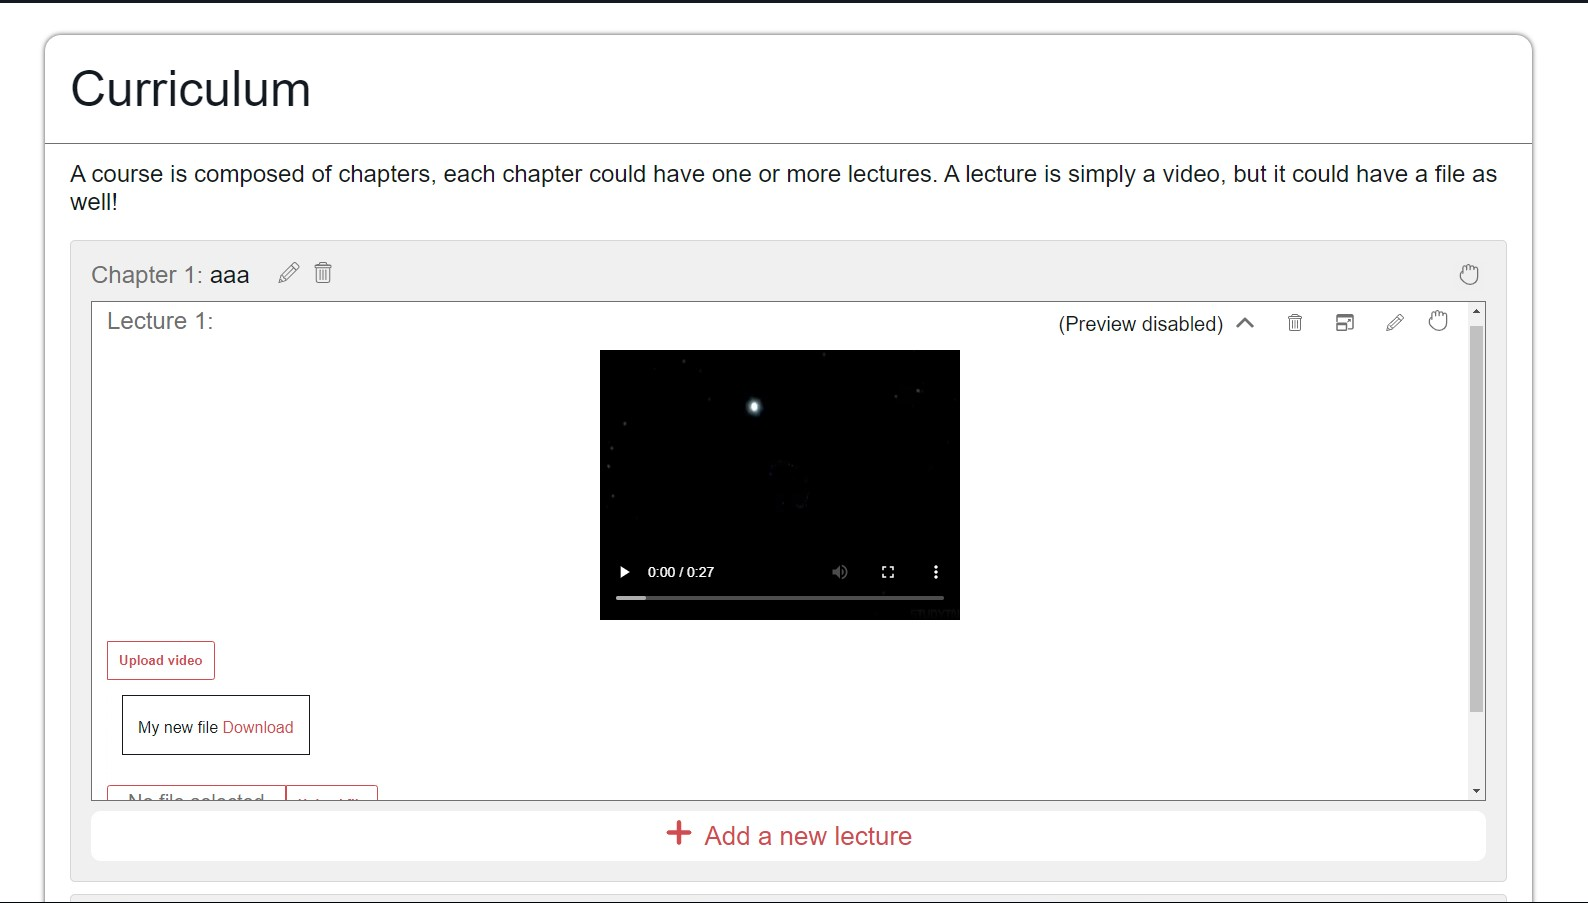
\includegraphics[width=150mm]{curriculum_form.jpg}
    \caption{Curriculum form interface}
    \label{fig:curriculum_form}
\end{figure}


\subsubsection{Landing page form}
In the landing page form, the user types the course info (title, subtitle, description...) and clicks the save button to update the course informations.

\vfill
\clearpage

\begin{figure}[!ht]
    \centering
    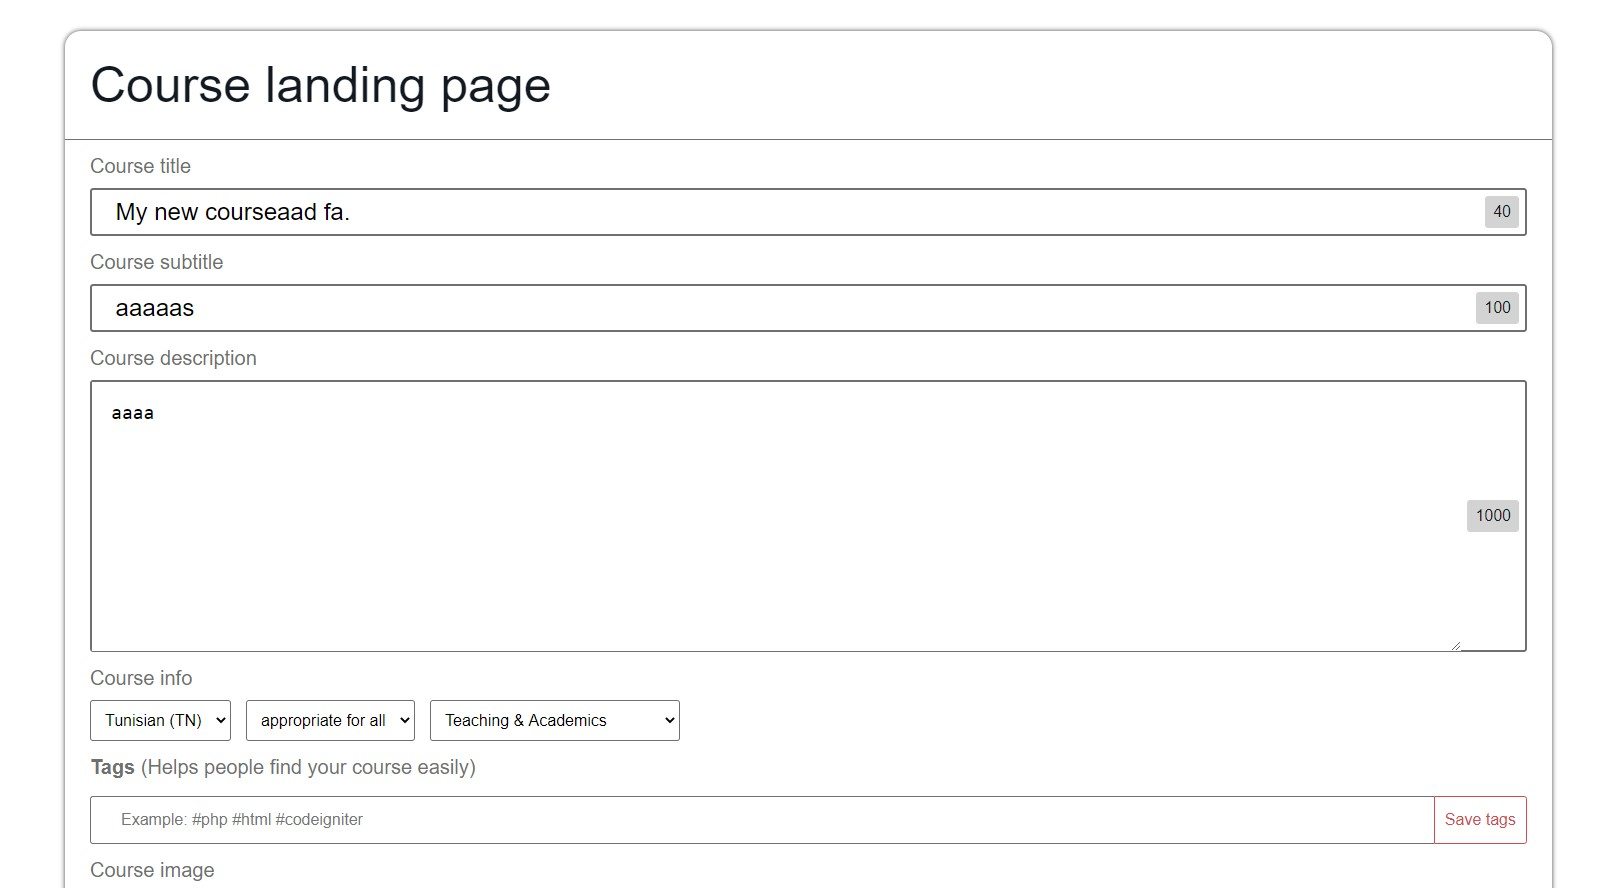
\includegraphics[width=150mm]{landing_page_form.jpg}
    \caption{Landing page form interface}
    \label{fig:landing_page_form}
\end{figure}


\subsubsection{Pircing form}
The instructor puts the price he wants in TND then clicks the save button to make a request to the server and update the price.

\begin{figure}[!ht]
    \centering
    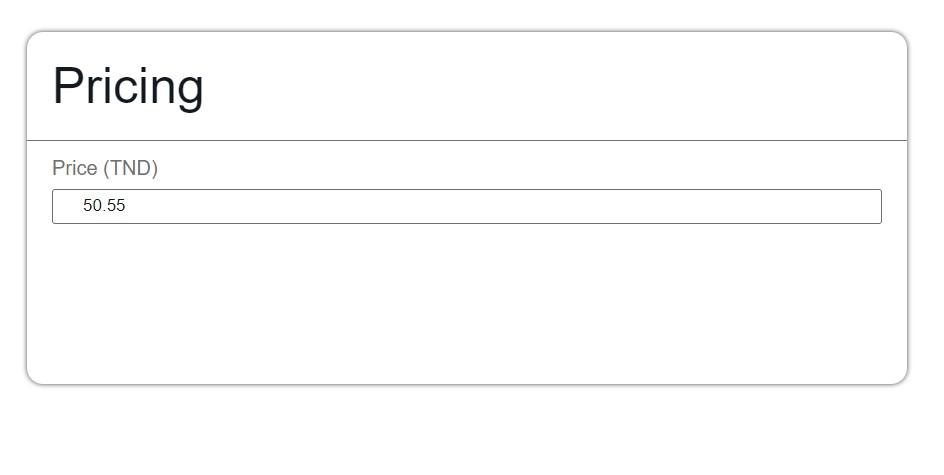
\includegraphics[width=150mm]{price_form.jpg}
    \caption{Pircing form interface}
    \label{fig:price_form}
\end{figure}

\vfill
\clearpage

\section*{Conclusion}
In this chapter, we coved how the instructor can manage his courses and access the dashboard.

\addcontentsline{toc}{section}{Conclusion}